
\chapter{TALEND Open Studio for Data Integration 5.6}

\section{Création du modèle OLAP}
\subsection{Question à répondre}
Analyse des ventes de bande dessinées d'une enseigne de librairie possédant plusieurs boutiques dans plusieurs villes.

\subsection{Modèle ROLAP}

L'implémentation ROLAP a été choisie par rapport au modèle MOLAP car même si la quantité de données était petite, il m'a semblé important d'étudier ce modèle qui paraît être très utilisé. Ne voyant rien justifier un modèle en flocon permettant de gagner de l'espace de stockage, j'ai utilisé un modèle en étoile.
La table de faits est la table vente. Les dimentsions sont le temps, la boutique(lieu d'achat), le client, et le livre. L'étoile est de type transaction.

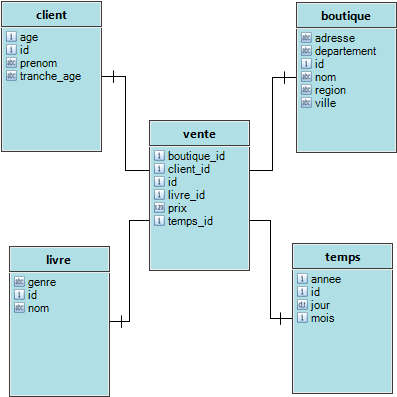
\includegraphics[clip=true, width=120mm, height=80mm]{images/Talend.png} 



\subsubsection{Table de faits vente}

\paragraph{Indicateurs}

prix de la vente; ce que le vente a rapporté

\subparagraph{fonctions d'agrégat}
\begin{itemize}
\item addition sur le prix
\item moyenne sur le prix
\end{itemize}


\paragraph{Dimension client}

\begin{itemize}
\item id
\item prenom
\item age
\item tranche\_age ("-12", "12-25", "35-65", "25-34", "+65")
\end{itemize}

\subparagraph{hiérarchie}
 age $<$ tranche\_age

\paragraph{Dimension boutique}
\begin{itemize}
\item id
\item nom
\item adresse
\item departement
\item ville
\item region
\end{itemize}

\subparagraph{hiérarchie}
adresse $<$ ville $<$ department $<$ region

\paragraph{Dimension livre}
\begin{itemize}
\item id
\item nom
\item genre
\end{itemize}

\subparagraph{hiérarchie}
nom $<$ genre

\paragraph{Dimension Temps}

\begin{itemize}
\item id
\item jour
\item mois
\item annee
\end{itemize}

\subparagraph{hiérarchie}
jour $<$ mois $<$ annee

\section{Intégration avec TALEND}

\subsection{Téléchargement Installation}
Le téléchargement se fait sur \url{http://fr.talend.com/download/data-integration}.
La documentation de l'outil est disponible au même endroit dans la partie Manuels d'utilisateurs et est facilement accessible.
L'outil est en fait basé sur Eclipse ce qui le rend facilement appréhendable pour ceux qui connaissent le célèbre IDE mais vient aussi avec ses défauts.

\subsection{Méthode utilisée}

Pour chaque dimension, j'ai essayé d'avoir un cas d'usage différent:
\begin{itemize}
\item La dimension livre se construit par une jointure classique entre deux tables. 
\item La dimension client est construite en utilisant la table client suivie d'une transformation sur l'un de ses champs afin de déduire la tranche d'age à partir de l'age.
\item La dimension boutique utilise des sources de données de type différents (CSV et postgres).
\item La dimension temps construite à partir de la table temps subit un action sur ses données afin d'enlever les doublons.
\end{itemize}

\subsection{Configuration des sources de données}
Le csv
\clearpage